\chapter*{序章\quad 電力変換はエネルギーの受け渡しである}
\addcontentsline{toc}{chapter}{序章\quad 電力変換はエネルギーの受け渡しである}
\markboth{序章}{序章}
\label{chap0}

スマートフォンの充電器は，コンセントの交流100\,Vを直流5\,Vに変える。
電気自動車はバッテリーの直流を交流に変えてモータを回し，
太陽光パネルの直流は交流に変えられて家庭や送電網へ流れ込む。
形は違っても，どれも「電力の形（電圧・周波数・直流か交流か）を目的に合わせて作り替える」装置であり，
この技術を\index{ぱわーえれくとろにくす@パワーエレクトロニクス}\textbf{パワーエレクトロニクス}という。

%%======================================================================
\section*{電力変換の地図}

電力の形は直流（DC）か交流（AC）かで分けられるから，変換は次の4種類しかない。
これが本書の地図である（\FIGref{fig0.1}）。

\begin{figure}[h]
\begin{center}
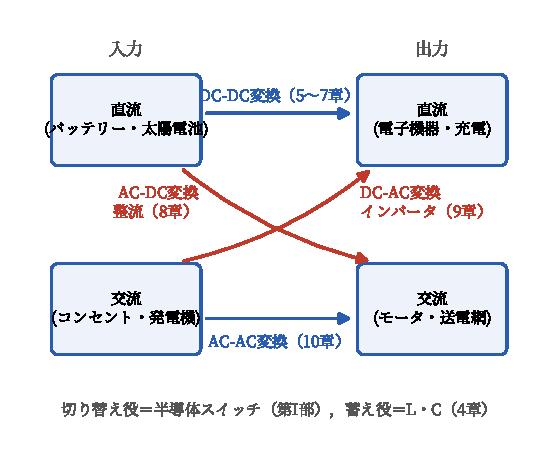
\includegraphics[clip]{figures/fig0.1.eps}
\end{center}
\caption{電力変換の地図。入力と出力の組合せで変換は4種類に分かれ，本書の第II部で順にすべてを扱う。
どの章にいても，この地図に立ち返れば現在地がわかる}
\label{fig0.1}
\end{figure}

\begin{箇条書}
\item \textbf{直流→直流}（DC-DC変換）：電圧の大きさを変える。5〜7章
\item \textbf{交流→直流}（AC-DC変換，整流）：コンセントから直流を作る。8章
\item \textbf{直流→交流}（DC-AC変換，インバータ）：バッテリーからモータや送電網へ。9章
\item \textbf{交流→交流}（AC-AC変換）：周波数や振幅を直接作り替える。10章
\end{箇条書}

%%======================================================================
\section*{本書を貫く1つの見方 ― エネルギーをどう蓄え，どう放出するか}

4種類の変換回路は，一見べつべつの回路に見える。
しかし根っこはすべて同じで，登場人物は3人しかいない。

\begin{screen}
\begin{enumerate}
\item \textbf{半導体スイッチ}：エネルギーの流れ道を高速に切り替える（第I部）
\item \textbf{インダクタ}：\textbf{磁場}にエネルギーを蓄え，\textbf{電流}を保とうとする（4章）
\item \textbf{キャパシタ}：\textbf{電場}にエネルギーを蓄え，\textbf{電圧}を保とうとする（4章）
\end{enumerate}
\end{screen}

スイッチが流れ道を切り替え，インダクタとキャパシタが
\textbf{エネルギーをいったん蓄えて，必要なときに放出する}。
降圧チョッパも，絶縁型コンバータも，インバータも，
「どこにエネルギーを溜め，いつ放出するか」が違うだけである。
本書はこの1つの見方ですべての変換回路を串刺しにする。
回路ごとに暗記するのではなく，共通の原理で理解してほしい。

%%======================================================================
\section*{なぜ「なぜ」から学ぶのか}

素子を回路記号として覚えるだけでも，回路を「読む」ことはできる。
しかし，いざ自分で「作る」段階では行き詰まる。
出力のリプルをどこまで抑えるか，素子にどこまで電圧をかけてよいか，なぜ発熱するのか ―
こうした設計の判断は，素子が\textbf{なぜそう振る舞うのか}を知ってはじめて下せるからである。

だから本書は遠回りに見えても，第I部で半導体スイッチを物理から解き明かす。
第1章の半導体の物理（バンドギャップ・絶縁破壊電界）が，
第3章でデバイスの性能（耐圧・損失・速度）を決め，
なぜワイドギャップ半導体（SiC・GaN）が注目されるのかまで，流行ではなく物理から説明できるようになる。

%%======================================================================
\section*{本書の約束}

\begin{screen}
\begin{enumerate}
\item \textbf{仮定を明示する。}電力変換の解析は「理想スイッチ・定常状態・リプルが小さい」といった仮定の上に成り立つ。
本書ではどの仮定を置いているかを毎回明示し，仮定が崩れるとどうなるか（不連続モードや損失）にも触れる。
教科書どおりにいかない実際の設計で，この習慣が効いてくる。
\item \textbf{公式は覚えるものではなく，導くもの。}数式の導出は途中を省略しない。
結果だけ使えばよい式は囲みで示す。
\item \textbf{手を動かして確かめる。}問・章末問題で導出や波形の描画を自分で行い，
回路シミュレータ\index{えるてぃーすぱいす@LTspice}\textbf{LTspice}で素子値を変えながら設計（リプル電流・リプル電圧）を確かめられる。
本書の回路はすべてLTspiceで再現でき，モデルファイルを配布する。
\end{enumerate}
\end{screen}

それでは，エネルギーの受け渡しの旅を始めよう。
まずは流れ道を切り替える主役 ― 半導体スイッチの正体からである。
